\documentclass{beamer}
\usepackage{amsmath, amsfonts}
\usepackage{listings}


\usepackage{amsmath, amsfonts}
\usepackage{listings}
\usepackage{xcolor}
\usepackage{graphicx}
\usepackage{booktabs}
\usepackage{tikz}
\usepackage{hyperref}
\usepackage{multicol}
\usepackage{lmodern}  
\usepackage{caption}
\usepackage{libertine}
\usepackage[libertine]{newtxmath}


\title[Enhanced Beamer Demo]{Hamilton Cycles and Elgenvalues of Graphs}
\author{Szymon Wojtulewicz}
\date{\today}

\usetheme{default}

\usefonttheme{professionalfonts}


\definecolor{accent}{RGB}{130,160,255}
\definecolor{blockbg}{RGB}{240,240,245}
\definecolor{blockborder}{RGB}{220,220,220}

\setbeamertemplate{navigation symbols}{}
\setbeamertemplate{footline}[frame number]
\setbeamertemplate{blocks}[default]


\setbeamercolor{block title}{fg=black,bg=blockbg}
\setbeamercolor{block body}{bg=blockbg}
% \setbeamerfont{block title}{series=\sffamily\bfseries}

\definecolor{codebg}{RGB}{250,250,250}
\definecolor{keywordcolor}{RGB}{70,110,200}
\definecolor{stringcolor}{RGB}{200,130,130}
\definecolor{commentcolor}{RGB}{140,180,140}

\lstset{
  backgroundcolor=\color{codebg},
  basicstyle=\ttfamily\footnotesize,
  keywordstyle=\color{keywordcolor}\bfseries,
  stringstyle=\color{stringcolor},
  commentstyle=\color{commentcolor}\itshape,
  frame=single,
  breaklines=true,
  showstringspaces=false,
  tabsize=2
}


\begin{document}

\frame{\titlepage}

\begin{frame}
  \centering
  \includegraphics[height=0.8\textheight,keepaspectratio]{img/main_paper.png}
\end{frame}


\begin{frame}{Outline}
  \tableofcontents
\end{frame}

\section{Prerequisites}
\subsection{Matrices of a graph}


\begin{frame}{Adjacency matrix}
  \begin{block}{}
    For a simple undirected graph \(G=(V,E)\) with vertices indexed \(1,\dots,n\), the adjacency matrix \(A_G\in\{0,1\}^{n\times n}\) has entries
    \[
      (A_G)_{i,j}=\begin{cases}
        1 & \text{if }\{i,j\}\in E,\\[4pt]
        0 & \text{otherwise}.
      \end{cases}
    \]
    In particular for a simple undirected graph $G$, \(A_G\) is symmetric and \((A_G)_{ii}=0\) for all \(i\).
  \end{block}
  \pause
  \vspace{0.5em}
  \begin{columns}[T,onlytextwidth]
    \begin{column}{0.55\textwidth}
      \centering
      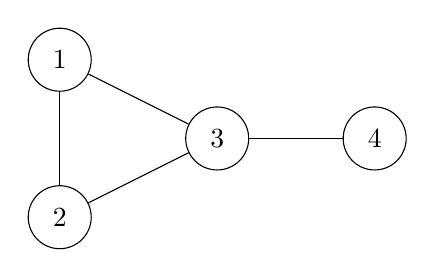
\begin{tikzpicture}[scale=1,auto,main node/.style={circle,draw,inner sep=1pt,minimum size=8mm}]
        \node[main node] (1) at (0,2) {1};
        \node[main node] (2) at (0,0) {2};
        \node[main node] (3) at (2,1) {3};
        \node[main node] (4) at (4,1) {4};
        \path
          (1) edge (2)
          (1) edge (3)
          (2) edge (3)
          (3) edge (4);
      \end{tikzpicture}
    \end{column}
    \begin{column}{0.45\textwidth}
      \[
      A_G=\begin{bmatrix}
      0 & 1 & 1 & 0\\
      1 & 0 & 1 & 0\\
      1 & 1 & 0 & 1\\
      0 & 0 & 1 & 0
      \end{bmatrix}
      \]

      \medskip

      Adjacency matrix \(A_G\) for vertices ordered $(1,2,3,4)$.
    \end{column}
  \end{columns}
\end{frame}

\begin{frame}{Degree matrix}
  \begin{block}{}
    For a graph \(G=(V,E)\) with vertices \(1,\dots,n\), the degree matrix \(D_G\in\mathbb{Z}^{n\times n}\) is diagonal with
    \[
      (D_G)_{i,j}=\begin{cases}
        \deg(i) & \text{if }i=j,\\[4pt]
        0 & \text{if }i\neq j.
      \end{cases}
    \]
  \end{block}
  \pause
  \vspace{0.5em}
  \begin{columns}[T,onlytextwidth]
    \begin{column}{0.55\textwidth}
      \centering
      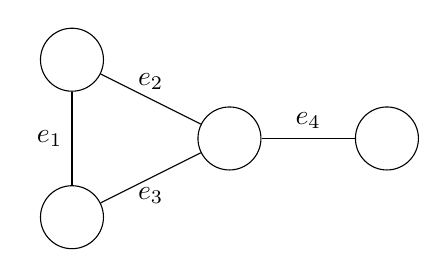
\begin{tikzpicture}[scale=1,auto,main node/.style={circle,draw,inner sep=1pt,minimum size=8mm}]
        \node[main node] (1) at (0,2) {};
        \node[main node] (2) at (0,0) {};
        \node[main node] (3) at (2,1) {};
        \node[main node] (4) at (4,1) {};
        \path
          (1) edge node[left]  {$e_1$} (2)
          (1) edge node[above] {$e_2$} (3)
          (2) edge node[below] {$e_3$} (3)
          (3) edge node[above] {$e_4$} (4);
      \end{tikzpicture}
    \end{column}
    \begin{column}{0.45\textwidth}
      \[
        D_G=\begin{bmatrix}
            2 & 0 & 0 & 0\\
            0 & 2 & 0 & 0\\
            0 & 0 & 3 & 0\\
            0 & 0 & 0 & 1
          \end{bmatrix}
      \]
    \end{column}
  \end{columns}
\end{frame}

\subsection{Eigen\{\text{values}, \text{vectors}\}}

\begin{frame}{Eigenvectors}
  \begin{block}{}
    For a matrix \(M_G\in\mathbb{R}^{n\times n}\), a scalar \(\lambda\in\mathbb{R}\) and a nonzero vector \(x\in\mathbb{R}^n\)
    form an eigenpair if
    \[
      M_G x = \lambda x.
    \]
  \end{block}
  \pause
  \vspace{0.5em}
  \[
    M_G=\begin{bmatrix}
      2 & 1 & 0\\[2pt]
      1 & 2 & 1\\[2pt]
      0 & 1 & 2
    \end{bmatrix},\qquad
    x=\begin{bmatrix}1\\[2pt]0\\[2pt]-1\end{bmatrix}.
  \]
  Verifying:
  \[
    M_G x = \begin{bmatrix}2\\[2pt]0\\[2pt]-2\end{bmatrix} = 2\,x,
  \]
  so \(x\) is an eigenvector of \(M_G\) with eigenvalue \(\lambda=2\). \\
  The remaining eigenvalues are \(2\pm\sqrt{2}\).
\end{frame}


\begin{frame}{Graph spectra}
  \begin{block}{}
    Consider the complete graph \(K_4\) on four vertices. 
    \[
      \operatorname{spec}(A_{K_4})=\{3,-1,-1,-1\},
    \]
    where the eigenvalue \(3\) has multiplicity \(1\) and \(-1\) has multiplicity \(3\).
  \end{block}
  \pause
  \vspace{0.5em}
  \begin{columns}[T,onlytextwidth]
    \begin{column}{0.55\textwidth}
      \centering
      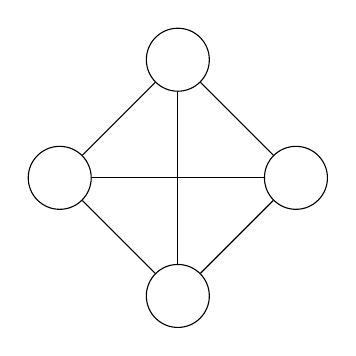
\begin{tikzpicture}[scale=1,auto,main node/.style={circle,draw,inner sep=1pt,minimum size=8mm}]
        \node[main node] (1) at (0,1.5) {};
        \node[main node] (2) at (1.5,0) {};
        \node[main node] (3) at (0,-1.5) {};
        \node[main node] (4) at (-1.5,0) {};
        \path
          (1) edge (2)
          (1) edge (3)
          (1) edge (4)
          (2) edge (3)
          (2) edge (4)
          (3) edge (4);
      \end{tikzpicture}
    \end{column}
    \begin{column}{0.45\textwidth}
      \[
        A_{K_4}=\begin{bmatrix}
          0 & 1 & 1 & 1\\
          1 & 0 & 1 & 1\\
          1 & 1 & 0 & 1\\
          1 & 1 & 1 & 0
        \end{bmatrix}
      \]

      \medskip

      Spectrum: \(\operatorname{spec}(A_{K_4})=\{3,-1,-1,-1\}\).
    \end{column}
  \end{columns}
\end{frame}

\subsection{Laplacian matrices}

\begin{frame}{Laplacian matrix}
  \begin{block}{}
    The Laplacian is defined as
    \[
      L_G = D_G - A_G.
    \]
  \end{block}
  \pause
  \vspace{0.5em}
  \begin{columns}[T,onlytextwidth]
    \begin{column}{0.45\textwidth}
      \centering
      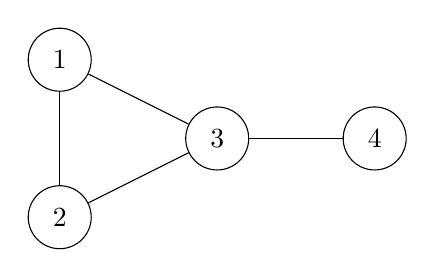
\begin{tikzpicture}[scale=1,auto,main node/.style={circle,draw,inner sep=1pt,minimum size=8mm}]
        \node[main node] (1) at (0,2) {1};
        \node[main node] (2) at (0,0) {2};
        \node[main node] (3) at (2,1) {3};
        \node[main node] (4) at (4,1) {4};
        \path
          (1) edge (2)
          (1) edge (3)
          (2) edge (3)
          (3) edge (4);
      \end{tikzpicture}
    \end{column}
    \begin{column}{0.55\textwidth}
      \[
        L_G = D_G - A_G = \begin{bmatrix}
          2 & -1 & -1 & 0\\
         -1 &  2 & -1 & 0\\
         -1 & -1 &  3 & -1\\
          0 &  0 & -1 & 1
        \end{bmatrix}
      \]

      \medskip
    \end{column}
  \end{columns}
\end{frame}

\begin{frame}{Signless Laplacian}
  \begin{block}{}
    The signless Laplacian is defined as
    \[
      Q_G = D_G + A_G.
    \]
  \end{block}
  \pause
  \vspace{0.5em}
  \begin{columns}[T,onlytextwidth]
    \begin{column}{0.55\textwidth}
      \centering
      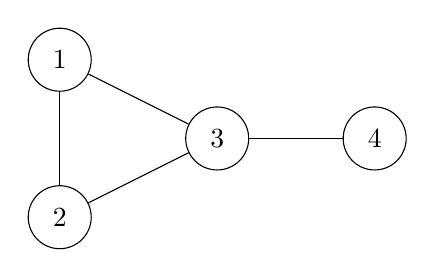
\begin{tikzpicture}[scale=1,auto,main node/.style={circle,draw,inner sep=1pt,minimum size=8mm}]
        \node[main node] (1) at (0,2) {1};
        \node[main node] (2) at (0,0) {2};
        \node[main node] (3) at (2,1) {3};
        \node[main node] (4) at (4,1) {4};
        \path
          (1) edge (2)
          (1) edge (3)
          (2) edge (3)
          (3) edge (4);
      \end{tikzpicture}
    \end{column}
    \begin{column}{0.45\textwidth}
      \[
        Q_G = D_G + A_G = \begin{bmatrix}
          2 & 1 & 1 & 0\\
          1 & 2 & 1 & 0\\
          1 & 1 & 3 & 1\\
          0 & 0 & 1 & 1
        \end{bmatrix}
      \]

      \medskip

    \end{column}
  \end{columns}
\end{frame}

\section{Main theorem}

\begin{frame}{Main theorem}
  \begin{block}{}
    If $M$ is an $n \times n$ symmetric matrix then we denote the eigenvalues of $M$ by $\lambda_i(M), i \in \{1, \dots, n\}$ with the order 
    \[
      \lambda_1(M) \leq \lambda_2(M) \leq \ \dots \ \leq \lambda_n(M)
    \]
  \end{block}
  \pause
  \begin{block}{Theorem 1.}
    Let $G$ be a graph on $n$ vertices and $C_n$ be an $n$-vertex cycle. If $G$ contains a Hamiltonian cycle, then for $i \in \{1, \dots, n\}$,
    \[
      \lambda_1(L_{C_n}) \leq \lambda_2(L_G) \text{ and } \lambda_1(Q_{C_n}) \leq \lambda_2(Q_G)
    \]
  \end{block}
\end{frame}

\subsection{Lemma 2.}

\begin{frame}{Hamiltonian cycle}
  \vspace{0.5em}
  \begin{center}
    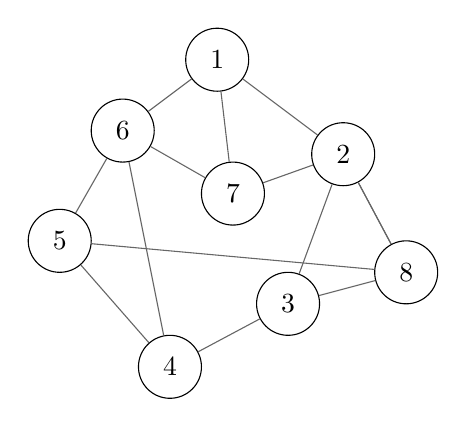
\begin{tikzpicture}[scale=1,auto,
        main node/.style={circle,draw,inner sep=1pt,minimum size=8mm,fill=white},
        other edge/.style={draw=black!60}
      ]
      % irregular positions
      \node[main node] (1) at (0,2.1)   {1};
      \node[main node] (2) at (1.6,0.9) {2};
      \node[main node] (3) at (0.9,-1.0)   {3};
      \node[main node] (4) at (-0.6,-1.8) {4};
      \node[main node] (5) at (-2.0,-0.2)  {5};
      \node[main node] (6) at (-1.2,1.2) {6};
      \node[main node] (7) at (0.2,0.4)  {7}; % moved to center
      \node[main node] (8) at (2.4,-0.6)  {8};

      % edges: mix of short and long-range chords
      \path[other edge]
        (1) edge (7)
        (1) edge (6)
        (1) edge (2)
        (2) edge (3)
        (2) edge (8)
        (3) edge (4)
        (3) edge (8)
        (4) edge (5)
        (4) edge (6)
        (5) edge (6)
        (5) edge (8)
        (6) edge (7)
        (7) edge (2)
        (8) edge (2);
    \end{tikzpicture}
  \end{center}
\end{frame}

\begin{frame}{Hamiltonian cycle}
  \vspace{0.5em}
  \begin{center}
    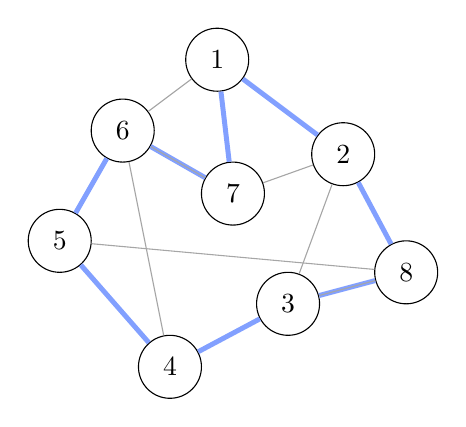
\begin{tikzpicture}[scale=1,auto,
        main node/.style={circle,draw,inner sep=1pt,minimum size=8mm},
        cycle edge/.style={draw=accent,line width=1.8pt},
        other edge/.style={draw=black!35}
      ]
      % same irregular positions
      \node[main node] (1) at (0,2.1)   {1};
      \node[main node] (2) at (1.6,0.9) {2};
      \node[main node] (3) at (0.9,-1.0)   {3};
      \node[main node] (4) at (-0.6,-1.8) {4};
      \node[main node] (5) at (-2.0,-0.2)  {5};
      \node[main node] (6) at (-1.2,1.2) {6};
      \node[main node] (7) at (0.2,0.4)  {7}; % moved to center
      \node[main node] (8) at (2.4,-0.6)  {8};

      % highlighted Hamiltonian cycle (nontrivial weaving)
      \path[cycle edge]
        (1) edge (2)
        (2) edge (8)
        (8) edge (3)
        (3) edge (4)
        (4) edge (5)
        (5) edge (6)
        (6) edge (7)
        (7) edge (1);

      % other edges (muted)
      \path[other edge]
        (1) edge (6)
        (2) edge (3)
        (3) edge (8)
        (4) edge (6)
        (5) edge (8)
        (6) edge (7)
        (7) edge (2);
    \end{tikzpicture}
  \end{center}
\end{frame}

\begin{frame}{}
  \begin{block}{Lemma 2.}
    Let $G$ be a graph on $n$ vertices and let $H$ be a subgraph of $G$ obtained by deleting an edge in $G$. Then
    \[
      \begin{aligned}
        0 &\le \lambda_1(L_H) \le \lambda_1(L_G) \le \lambda_2(L_H) \le \lambda_2(L_G) \le \cdots \\
          &\le \lambda_{n-1}(L_G) \le \lambda_n(L_H) \le \lambda_n(L_G)
      \end{aligned}
    \]
    and
    \[
      \begin{aligned}
        0 &\le \lambda_1(Q_H) \le \lambda_1(Q_G) \le \lambda_2(Q_H) \le \lambda_2(Q_G) \le \cdots \\
          &\le \lambda_{n-1}(Q_G) \le \lambda_n(Q_H) \le \lambda_n(Q_G)
      \end{aligned}
    \]
  \end{block}
\end{frame}

\subsection{Proof outline}
\begin{frame}{Incidence matrix}
  
  \begin{block}{}
    The incidence matrix of $G$, denoted $P_G$ is the $|V(G)| \times |E(G)|$ matrix with entries
    \[
      (P_G)_{u,e}=\begin{cases}
        1 & \text{if $u$ and $e$ are incident} \\
        0 & \text{otherwise}.
      \end{cases}
    \]
  \end{block}
  \pause
  \vspace{0.5em}
  \begin{columns}[T,onlytextwidth]
    \begin{column}{0.55\textwidth}
      \centering
      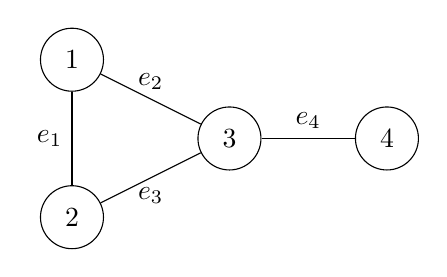
\begin{tikzpicture}[scale=1,auto,main node/.style={circle,draw,inner sep=1pt,minimum size=8mm}]
        \node[main node] (1) at (0,2) {1};
        \node[main node] (2) at (0,0) {2};
        \node[main node] (3) at (2,1) {3};
        \node[main node] (4) at (4,1) {4};
        \path
          (1) edge node[left]  {$e_1$} (2)
          (1) edge node[above] {$e_2$} (3)
          (2) edge node[below] {$e_3$} (3)
          (3) edge node[above] {$e_4$} (4);
      \end{tikzpicture}
    \end{column}
    \begin{column}{0.45\textwidth}
      \[
        B_G=\begin{bmatrix}
          1 & 1 & 0 & 0\\
          1 & 0 & 1 & 0\\
          0 & 1 & 1 & 1\\
          0 & 0 & 0 & 1
        \end{bmatrix}
      \]

      \medskip

      Incidence matrix \(B_G\) for vertices $(1,2,3,4)$ and edges $(e_1,e_2,e_3,e_4)$.
    \end{column}
  \end{columns}
\end{frame}

\begin{frame}{Oriented incidence matrix}
  \begin{block}{}
    For a chosen orientation of a graph \(G\). The oriented incidence matrix \(K_G\in\{-1,0,1\}^{n\times m}\) has entries
    \[
      (K_G)_{v,e}=\begin{cases}
        1 & \text{if }v\text{ is the terminal vertex of }e,\\
        -1 & \text{if }v\text{ is the initial vertex of }e,\\
        0 & \text{otherwise.}
      \end{cases}
    \]
  with respect to the orientation.
  \end{block}
  \pause
  \vspace{0.5em}
  \begin{columns}[T,onlytextwidth]
    \begin{column}{0.55\textwidth}
      \centering
      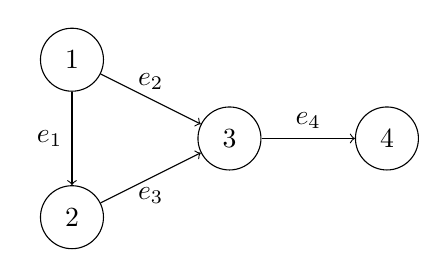
\begin{tikzpicture}[scale=1,auto,main node/.style={circle,draw,inner sep=1pt,minimum size=8mm}]
        \node[main node] (1) at (0,2) {1};
        \node[main node] (2) at (0,0) {2};
        \node[main node] (3) at (2,1) {3};
        \node[main node] (4) at (4,1) {4};
        % orientations: e1:1->2, e2:1->3, e3:2->3, e4:3->4
        \path
          (1) edge[->] node[left]  {$e_1$} (2)
          (1) edge[->] node[above] {$e_2$} (3)
          (2) edge[->] node[below] {$e_3$} (3)
          (3) edge[->] node[above] {$e_4$} (4);
      \end{tikzpicture}
    \end{column}
    \begin{column}{0.45\textwidth}
      \[
        K_G=\begin{bmatrix}
         -1 & -1 &  0 &  0\\
          1 &  0 & -1 &  0\\
          0 &  1 &  1 & -1\\
          0 &  0 &  0 &  1
        \end{bmatrix}
      \]

      \medskip

    \end{column}
  \end{columns}
\end{frame}

\begin{frame}{Proof outline}
  \begin{block}{}
    \[
      L_G = K_G K_G^{\!T},\qquad Q_G = P_G P_G^{\!T},
    \]
    \(K_G\) depends on the chosen orientation, while \(L_G\) does not.
  \end{block}
  \pause
  \begin{block}{}
    For any matrix \(N\) the matrices \(N N^{T}\) and \(N^{T}N\) are symmetric positive semidefinite. \\ 
    Apart from multiplicities of the eigenvalue \(0\) their nonzero spectra coincide. \\
    Hence the positive eigenvalues of \(L_G\) agree with the positive eigenvalues of \(K_G^{T}K_G\), and similarly for \(Q_G\) and \(P_G^{T}P_G\).
  \end{block}
\end{frame}

\begin{frame}{Proof outline}
  \vspace{-0.8em}
  \begin{block}{}
    \[
      L_G = K_G K_G^{\!T},\qquad Q_G = P_G P_G^{\!T},
    \]
    \(K_G\) depends on the chosen orientation, while \(L_G\) does not.
  \end{block}
  \begin{block}{}
  The spectra of $L_G$ and $Q_G$ match the spectra of \(K_G^{T}K_G\) \(P_G^{T}P_G\) almost entirely.
  \end{block}
  \pause
  \begin{block}{}
    Let \(H\) be a subgraph of \(G\) obtained by deleting an edge from \(G\). Then the matrix \(K_H^{T}K_H\) is obtained from \(K_G^{T}K_G\) by deleting the row and column corresponding to the deleted edge, and \(P_H^{T}P_H\) is obtained from \(P_G^{T}P_G\) in a similar way. 
  \end{block}
  \pause
  \begin{block}{}
    Use the interlacing properties of principal submatrices of symmetric matrices to prove the lemma.
  \end{block}
\end{frame}

\begin{frame}{Proof outline}
  \begin{block}{Lemma 2.}
    Let $G$ be a graph on $n$ vertices and let $H$ be a subgraph of $G$ obtained by deleting an edge in $G$. Then
    \[
      \begin{aligned}
        0 &\le \lambda_1(L_H) \le \lambda_1(L_G) \le \lambda_2(L_H) \le \lambda_2(L_G) \le \cdots \\
          &\le \lambda_{n-1}(L_G) \le \lambda_n(L_H) \le \lambda_n(L_G)
      \end{aligned}
    \]
    and
    \[
      \begin{aligned}
        0 &\le \lambda_1(Q_H) \le \lambda_1(Q_G) \le \lambda_2(Q_H) \le \lambda_2(Q_G) \le \cdots \\
          &\le \lambda_{n-1}(Q_G) \le \lambda_n(Q_H) \le \lambda_n(Q_G)
      \end{aligned}
    \]
  \end{block}
\end{frame}

\begin{frame}{Main theorem}
\begin{block}{Theorem 1'.}
  Let $G$ be a graph on $n$ vertices and $m$ edges. Suppose $G$ contains a Hamilton cycle. Then for $i=1,\dots,n$,
  \[
  \lambda_i(L_{C_n}) \le \lambda_i(L_G)
  \qquad\text{and}\qquad
  \lambda_i(Q_{C_n}) \le \lambda_i(Q_G).
  \]
  \pause
  In addition, if $m<2n$, then for $i=m-n+1,\dots,n$,
  \[
  \lambda_{\,i-m+n}(L_G) \le \lambda_i(L_{C_n}) \le \lambda_i(Q_G)
  \]
  and
  \[
  \lambda_{\,i-m+n}(Q_G) > \lambda_i(Q_{C_n}) \le \lambda_i(L_G).
  \]
  \end{block}
\end{frame}

\subsection{Usecase}
% \begin{frame}{}
%   \begin{block}{Corollary 3.}
%     Let $G$ be a $k$-regular graph on $n$ vertices. If $G$ contains a
%     Hamilton cycle, then for $i=1, \dots, n$,
%     $$
%     \lambda_{i}(A_{G}) - (k-2) \le \lambda_{i}(A_{C_{n}}) \le \lambda_{i}(A_{G}) + (k-2).
%     $$
%   \end{block}
  
% \end{frame}

\begin{frame}{A non-hamiltonian graph}
  \begin{block}{The 1-tough bipartite graph containing a 2-factor}
    
  \end{block}
  \centering
    \includegraphics[height=0.5\textheight,keepaspectratio]{img/graph.png}
\end{frame}

\end{document}
